\chapter{Vector Embedding}

Transformers builded in 2017 after the famous google's paper “attention is all you need”.
Embeddings: advanced reprersentations to reppresents words/tokens in a vectors in a dense ways with limited numbers of dimensions ~300 dims.
We would like to have:
semenatic meaning of a world
relationsheep among words, worlds with similar connections are linked via similar transformers

\begin{figure}[h!]
  \centering
  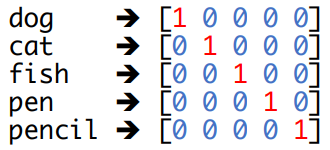
\includegraphics[width=0.3\linewidth]{content/Parts/images/2026-09-28-09-35-11.png}
\end{figure}

\section{One-Hot encoding}
One-hot encoding was used before embeddings. Vocaboly of 5 words with 5 dimension vector and set 0s and only one 1 each word.
Disadvantages:
This approach is sparse, dimensions = words count, not feasible.
Not preservation of similarity and no relationship among words. Vector are orthogonal.
\section{Distributed representation}
We distribute the sematic word across all the dimension.
But how do we figure it the vector? We use NN model to learn there words and create this vectors.
E.g. I use a …. to write the essay. We ask the model to predict the blank, this encourage the model to figure it out, starting the surrounded words, context.
Can we figuire out the probability of each vocabulary, based on the context?
Some step to

\begin{itemize}
  \item assign a vector for each words in the context, at beginning is random number
  \item Take all of this vector and aggregate all vectors and sum them up (\textbf{context vector})
\end{itemize}

Context vector and vector of all possible words.

Cosine similarity = cross entropy → gradient descent → backpropagation → update the vectors to make the loss function go dow.
In this is reaped for millions of sentences.
Pence or pencil now are similar and connected, semantic related, now two word can have same number, but it is fine.

\section{In terms of matrices}
We need to compute a matrix moltiplication. All vectors for input words can be staked into matrix.


This was presented in a paper of 2000. Then in the 2014, thirty years later.
\section{Limitation of WordToVec}

\begin{itemize}
  \item Cannot manage words are not in the vocabulary, OOV (out of vocabulary)
  \item This vector are not contextualized
\end{itemize}

After the tranign, the vector is the same, and during the infference some word depends on
the context, e.g. bank (river or money).


\section{FastText}

Allows to figure out some new words. Braking up words into subwords. E.g. <where> -->  <wh, whe, her, ere, re>
Insufficeint, the "in" has different meaning between two words and the prefixes of a word.

Does this works well? Not the perfect solution.


\section{Visualizations - Semantic meanings}
Reducing to 2 dimensions with Principal
Component Analysis (for visualization
purposes). The words belonging to the 3 categories are
well-separated in the “compressed” embedding space


\section{Inside an RNN}
We have three dense NN layers. Two input and two output.

\begin{itemize}
  \item \textbf{Input layer}: processes the current input,
        produces a vector with the same dimensionality as the hidden state. Makes the input
        and the state the same size dimentionality
  \item \textbf{State layer}: processes the hidden state from
        the previous step

  \item \textbf{Output layer}: Summed the two vectors and produces
\end{itemize}

\subsection{Weight sharing}

\subsubsection{Backpropagation-through-time}



\section{Encoder-decoder architecture}

Ideally, the model should:

\begin{itemize}
  \item See the entire sequence before starting generating the output
\end{itemize}


\begin{center}
  \begin{minipage}{0.65\linewidth}
    
  \end{minipage}%
  \hfill
  \begin{minipage}{0.3\linewidth}
    \centering
    \includegraphics[width=0.3\linewidth]{content/Parts/images/images/2026-09-28-11-13-30.png}
  \end{minipage}
\end{center}


